\documentclass{book}

\usepackage{graphicx,xcolor}
\usepackage{wrapstuff}

\graphicspath{{media/}}

\title{Fear Driven Development Manifesto}
\date{\the\year}
\author{Anon}

\newcommand{\myquote}[1]{
    \makebox[\textwidth][c]{
    \begin{minipage}{8cm}
        \emph{
            ``#1''
        }
    \end{minipage}
    }
    \\

}

\newcommand{\principle}[2]{
    % The formatting is somewhat fucked
    \fcolorbox{black}{gray!30}{
    \begin{minipage}{10cm}
        \raisebox{-.3\baselineskip}{
            
\includegraphics[
                height=\baselineskip,
                width=\baselineskip,
                keepaspectratio,
            ]{principle.png}#2
        }
        {\bf Fear Driven principle:}

        #1
    \end{minipage}
    }
    \\
}

\begin{document}
    \maketitle

    \myquote{
        We are uncovering better ways of developing
        software everyday
        by arguing and
        excluding others from doing it.
    }

    The software ecosystem values processes and tools
    over individuals.
    This practice is dehumanizing and highly immoral.
    Machines will never be able to code,
    hence development must be treated as an inherently human activity.
    We hold this truth self-evident,
    that feelings are the most remarkable aspect of the human experience,
    granted by our Creator\footnote{Hail Satan},
    and amongst them fear is the most prevalent.

    \begin{figure}[h!]
        \centering
        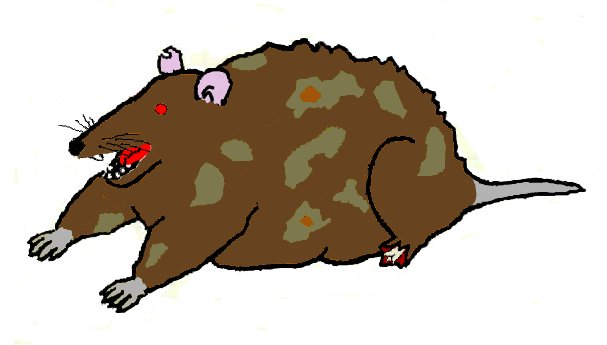
\includegraphics[width=40mm]{keith.jpeg}
        \caption{Overall process}
        \label{fig:method}
    \end{figure}

    As the vision of the industry fades, % NOTE: "if the carrot does not work, use a stick."
    we must branch.
    We propose a system
    --as spiritual as physical--
    where fear is allowed to manifest,
    not only in its full really,
    but creating its own definitive reality.
    We call this Fear Driven Development,
    or FDD for short.

    Bellow are the core principles of FDD:
    \begin{enumerate}
        \item Fear is key
        \item There is no mistake which cannot be punished, no matter how minuscule it is % XXX: should not be?
        \item Brutalization is a social construct
        \item No developer is irreplaceable
        \item Languages are irreplaceable
        \item Frameworks must be replaced\footnote{Always and without end}
        \item Monitoring increases productivity
        \item Programming is about following the rules
        \item Copyright is in the quantum state of only existing while being enforced
        \item x is the baseline % NOTE: this one MUST be the 10th
        \item Progress is exponential and will never stop,
               yet we shall live in dreadful doubt
        % XXX:
        % > the 12th can be bought following the qr code below
        % cool, but what is a funny qr code? rickrolling would feel cheap
    \end{enumerate}

    We firmly believe FDD is a rightful heir to TDD/AGILE
    and the next logical step in the evolution of programming.
    Consequently,
    there are many previous practices that we adore and endorse,
    with slight modifications perhaps.

    The daily ritual of cargo-culting is already a
    software engineering miracle.
    Its essence must be gripped and amplified.
    Take a personalized path,
    a slow, yet firm start would be
    to utter the name of Baal during each Java import,
    or perhaps starting on the deep end,
    you could sacrifice a goat during every daily stand-up.
    The later is truly desirable as it propagates the revolution.
    The more Fear Driven Developers we have,
    the more we all are going to make it.
    % XXX: this reference to OOP pseudo-intellectual bullshit should
    %       expanded in its own paragraph?
    Remember more eyes see more things and
    Fear Driven techniques are not invented,
    but discovered.
    \\

    % --- Expanding on:
    %  "Fear is key"

    System stress testing is standard procedure nowadays,
    and what could be a
    more complex or higher liability system
    than the developer team itself?

    Remember: the only way to avoid unexpected catastrophic failure
    is to cause it.
    Our creating will must say: "But thus would I have it."
    % XXX: a "cope" pun is REQUIRED here (coperate?)
    % -- honestly im not sure anymore, if feels forced
    \\

    \principle{
        An Art Of Not Coding must to be established,
        liberating us from all bugs
        and creating the simplest design imaginable.
    }{
        \footnote{Yin \& Yang illustrated in Gimp}
    }

    It is said that a developer in the \emph{zone} holds
    inhumane power at their finger tips.
    That's dangerous.
    By definition,
    its possible effects on our stocks is incalculable by humans
    and our Diagonal-11 has yet to halt on the problem.

    It might take as little as 5 minutes to arrive to the \emph{zone},
    but a single well targeted email may torpedo their whole day.

    Similarly talking to them may terrify their putrid souls yet more.
    If you haven't yet, you could either become or employ a dedicated
    boogeyman to this end.
    As a clever way to add insult to injury
    (which is to be endorsed),
    you could call this position something vague and childish.
    For example the KUDOS Emperor of the Abstraction Wizards.
    Better yet, KEAW.
    The more layers of (linguistic) indirection, the better.

    Alternatively,
    if you would prefer not to torture your subordinates\footnote{due to economic reasons},
    you could make them torture each other.

    A frustrated programmer is a toxic programmer.
    With this observation only,
    our possibilities became endless.

    Something as miniscule as forcing them to use inadequate tools
    tends to wear them down over time.

    Which could only be more brilliant of Excel had its own, separate shares.
    Especially since the murders stopped.
    \\

    \fcolorbox{black}{gray!10}{
    \begin{minipage}{10cm}
        \begin{center}
            {\bf The Daily News }
        \end{center}
        \hrule
        \vspace{0.3em}
        \begin{wrapstuff}[l]
            
\includegraphics[width=1cm]{dropkicker.jpeg}
        \end{wrapstuff}
        %{\bf The infamous Dropkick Killer has been arrested!} % NOTE: i hate latex
        \textbf{The infamous Dropkick Killer has been arrested!}
        He has been apprehended on a deserted island.
        Authorities caught the killer while he was manhunting an innocent victim,
        driven by a relentless pursuit that lasted four days.
        Deprived of food and water,
        the killer made the crucial mistake of opening Tor,
        while he was the only one running it in the area.
    \end{minipage}
    }
    \\

    Another crucial angle of attack is the documentation.
    Incomprehensive documentation is important % NOTE: "Working software over 
    to any proof of concept software.          %        comprehensive documentation"
    Communication\footnote{and mostly the lack thereof}
    is only an adequate alternative
    until the death of the maintainer,
    even if we bus factor in the temporal Fear Driven Development of Death.
    
    Regardless there are concrete improvements to be had
    in the quality of documentation projects tend to produce\footnote{
        With a big IF assuming they do.
    }.

    In our observations,
    out of the 4 types we differentiate,
    usually only 1 is available:
    \begin{itemize}
        \itemsep-0.5em 
        \item Reference
        \item Developer Guide
        \item User Guide
        \item Contributor Guide
    \end{itemize}
    This approach successfully angers most,
    but there are better alternatives.
    % NOTE to emil: how the fuck do i stop using "but"s/"however"s to transition between topics?
    %               i seem to be conceptually incapable, like as if i was missing
    %                some higher level understanding of english and compensating on a word level.

    The most prevalent was developed by Mozilla\footnote{
        The same company that gifted Rust to the Fear Driven community.
    },
    where categories are combined and partial.
    This way,
    people looking for concise definitions will have to read tutorials
    and the ones looking for basic help will have to consult tables.
    The name we suggest for this type of documentation is
    "Documenation As For Identitfy Crysis"\footnote{
        or DAFIC for short; remember: insult to injury!
    }.
    \\

    These all are great tools to the unlock the true potential of Fear Driven Development,
    envisioned below.
    \\

    \begin{figure}[h!]
        \centering
        
\includegraphics[width=40mm]{angry-pink-wojak.png}
        \caption{True potential of Fear Driven Development}
        \label{fig:method}
    \end{figure}

    % --- Expanding on:
    %  "There is no mistake which cannot be punished, no matter how minuscule it is"

    Footguns are the scariest spooks;
    the most potent conception of absolute terror,
    absolute power,
    and absolute evil ever conceived by the human mind.
    Footguns are the power that overcome all human probabilities
    and transcend even the greatest possibilities.
    \\

    \myquote{
        No deed can be annihilated: how could it be undone by the penalty! This,
        this is what is eternal in the 'existence' of penalty, that existence also must be
        eternally recurring deed and guilt!
    }

    But would it be even better if footguns actually existed?

    A simple contraption really.
    A standard .22 firearm attached directly to stderr
    with a simple string.
    This instrument of torture can strike anxiety
    to the heart of any programmer while only
    damaging his second least used body part,
    which most crucially is not required for work.
    Of course every team is different,
    you may have to adjust the caliber for example.
    We advise experimentation.
    \\

    % --- Expanding on:
    %  "Brutalization is a social construct"
    It is estimated that casinos lose 300 billion dollars
    every year to poker card counters.  % NOTE: bullshit statistic
    They counter it by throwing the cheaters out.
    Would it not be logical then for the software industry to do the same?

    \principle{
        % --- Expanding on:
        %  "Programming is about following the rules"
        Rules must be followed.
        Rules not being followed is called hacking, which is illegal;
        regardless of what some group which is unable to decide
        whether they are a hot beverage thinks. %NOTE:  aM I Tea?
    }{}

    By slightly tweaking the rules of planning poker and
    investing as little as \$200, it is possible.
    \\

    \begin{figure}[h!]
        \centering
        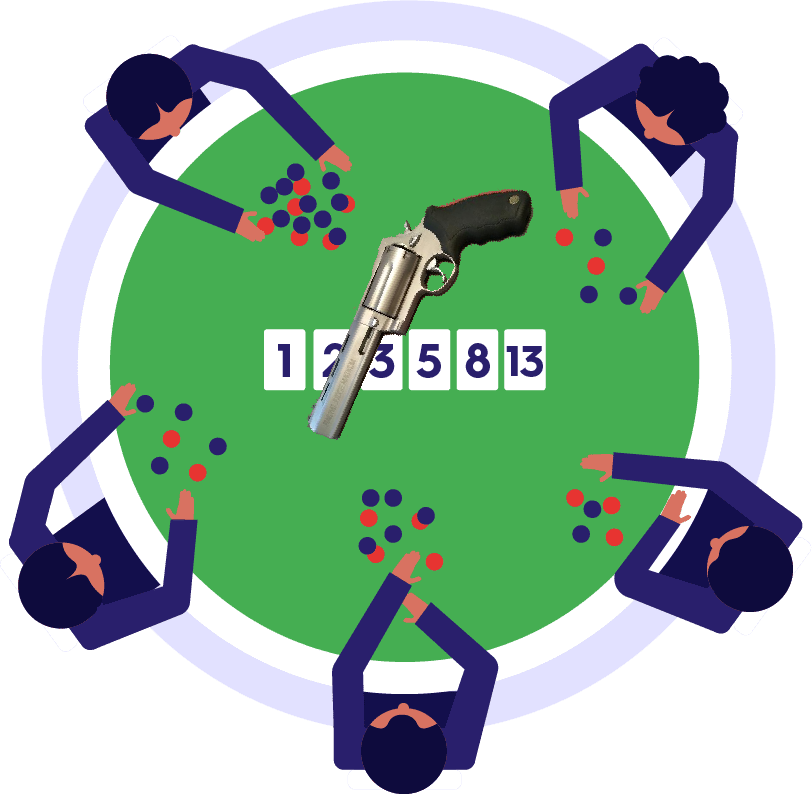
\includegraphics[width=50mm]{planning-russian-roulette.png}
        \caption{Planning Russian Roulette}
        \label{fig:method}
    \end{figure}

    % --- Expanding on:
    %  "No developer is irreplaceable"
    After good meeting,
    the tree of the job market has been watered with
    the blood of developers and managers.

    This means an opportunity give more work to HR.
    \\

    \principle{
        more work done === higher productivity
    }{}

    % --- Expanding on:
    %  "Languages are irreplaceable"
    Our new developers however must
    carefully selected.
    Every company can safely assume that candidates
    already gain years of experience at other companies,
    thus its fair to include that in the job requirements.
    One exception might be those positions regarding
    our critical infrastructure running on
    COBOL\footnote{Dictionary entries near COBOL: "cocaine"},
    as the education of bachelors is usually perfectly
    up to date.

    \begin{figure}[h!]
        \centering
        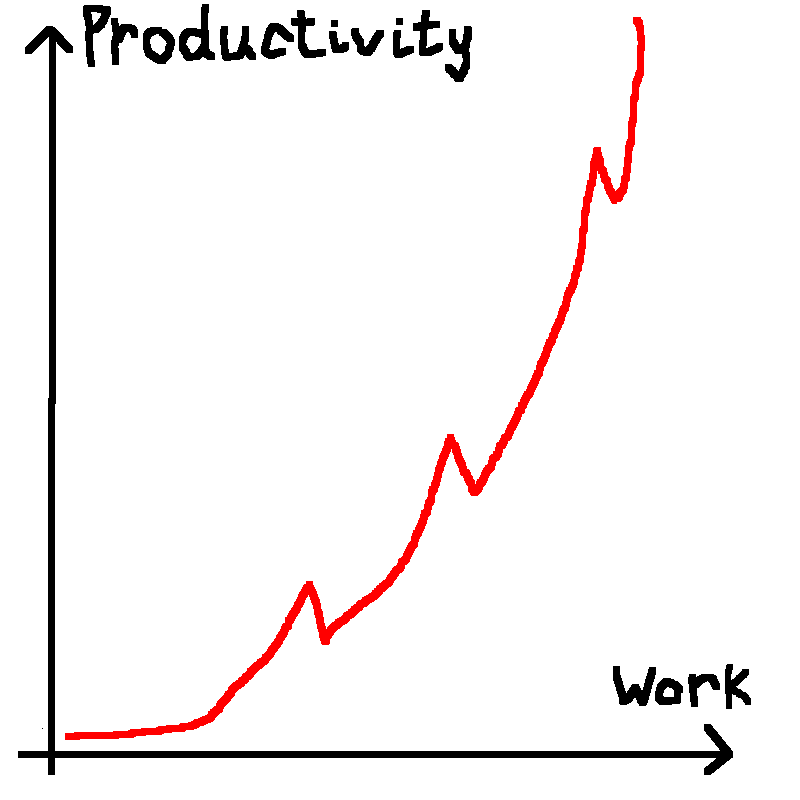
\includegraphics[width=35mm]{productivity_work.png}
        \caption{Our trustworthy statistics}
        \label{fig:method}
    \end{figure}

    % --- Expanding on:
    %  "Copyright is in the quantum state of only existing while being enforced"
    Whenever the team is ready to start developing,
    grand and powerful choices will have to be made.
    \vspace{0.5em}

    \principle{
        The most important components of any software are the License and the Code of Conduct
    }{}

    The fear to release any source code,
    because the quality being public might permanently damage your brand
    or it may increase the productivity of a similar group
    by 0.1\% on the other side of the planet,
    is as pure of a fear as any.
    Embrace it.

    However another option would be choosing open source licenses out of PR considerations
    and or to attempt piggy backing on added free labour\footnote{
        this later tends not to work out,
        as most who would have the free time to contribute
        are busy developing their programming language
        so they may write a game engine one day,
        so they may write a game one day.
    }.
    What is important to keep in mind while making a pick, is that GPLv3\footnote{
        without the 'A' of course
    }
    has a large appeal,
    but so does restricting distribution in Russia using GPLv2.
    \\

    % --- Expanding on:
    %  "Progress is exponential and will never stop,
    %    yet we shall live in dreadful doubt"
    \textbf{
        Now, you know everything to become a successful Fear Driven Developer.
        Godspeed and praise the straight lines on a graph!
    }

\end{document}

#############
### NOTES ###
#############

implied\_meaning\_of\_fdd:
    >pro FAGMAN satanism
    >developer exploitation
    >trying to force better results without better education or tools

emilemilemil | Fear driven development creates 0% of the programs in production,
thereby creating a astronomic 0% of bugs.

SUICIDE NOTE QUOTE
God is the greatest greatness; the most potent conception
of absolute perfection, absolute power, and absolute
goodness ever conceived of by the human mind. The
conception of God is being beyond all conception. God is the
power that overcomes all human probabilities and
transcends even the greatest possibilities.
But would it be even better if God actually existed?

ORIGINAL AGILE BULLSHIT

Manifesto for Agile Software Development

We are uncovering better ways of developing
software by doing it and helping others do it.
Through this work we have come to value:

Individuals and interactions over processes and tools
Working software over comprehensive documentation
Customer collaboration over contract negotiation
Responding to change over following a plan

That is, while there is value in the items on
the right, we value the items on the left more.

Principles behind the Agile Manifesto

We follow these principles:

Our highest priority is to satisfy the customer
through early and continuous delivery
of valuable software.

Welcome changing requirements, even late in
development. Agile processes harness change for
the customer's competitive advantage.

Deliver working software frequently, from a
couple of weeks to a couple of months, with a
preference to the shorter timescale.

Business people and developers must work
together daily throughout the project.

Build projects around motivated individuals.
Give them the environment and support they need,
and trust them to get the job done.

The most efficient and effective method of
conveying information to and within a development
team is face-to-face conversation.

Working software is the primary measure of progress.

Agile processes promote sustainable development.
The sponsors, developers, and users should be able
to maintain a constant pace indefinitely.

Continuous attention to technical excellence
and good design enhances agility.

Simplicity--the art of maximizing the amount
of work not done--is essential.

The best architectures, requirements, and designs
emerge from self-organizing teams.

At regular intervals, the team reflects on how
to become more effective, then tunes and adjusts
its behavior accordingly. 
